\let\negmedspace\undefined
\let\negthickspace\undefined
\documentclass[journal]{IEEEtran}
\usepackage[a5paper, margin=10mm, onecolumn]{geometry}
%\usepackage{lmodern} % Ensure lmodern is loaded for pdflatex
\usepackage{tfrupee} % Include tfrupee package

\setlength{\headheight}{1cm} % Set the height of the header box
\setlength{\headsep}{0mm}     % Set the distance between the header box and the top of the text

\usepackage{gvv-book}
\usepackage{gvv}
\usepackage{cite}
\usepackage{amsmath,amssymb,amsfonts,amsthm}
\usepackage{algorithmic}
\usepackage{graphicx}
\usepackage{textcomp}
\usepackage{xcolor}
\usepackage{txfonts}
\usepackage{listings}
\usepackage{enumitem}
\usepackage{mathtools}
\usepackage{gensymb}
\usepackage{comment}
\usepackage[breaklinks=true]{hyperref}
\usepackage{tkz-euclide} 
\usepackage{listings}
% \usepackage{gvv}                                        
\def\inputGnumericTable{}                                 
\usepackage[latin1]{inputenc}                                
\usepackage{color}                                            
\usepackage{array}                                            
\usepackage{longtable}                                       
\usepackage{calc}                                             
\usepackage{multirow}                                         
\usepackage{hhline}                                           
\usepackage{ifthen}                                           
\usepackage{lscape}
\begin{document}

\bibliographystyle{IEEEtran}

\title{5.2.24}
\author{EE25BTECH11021 - Dhanush sagar}
% \maketitle
% \newpage
% \bigskip
\maketitle \vspace{-1cm}
\renewcommand{\thefigure}{\theenumi}
\renewcommand{\thetable}{\theenumi}
\setlength{\intextsep}{10pt} % Space between text and floats

\
\numberwithin{figure}{enumi}
\renewcommand{\thetable}{\theenumi}

\textbf{Question:} \\
Solve the following system of linear equations\\

px + qy = p - q \\
qx - py = p + q \\


\textbf{Solution:} \\
Given
\begin{align}
px + qy &= p - q \\
qx - py &= p + q
\end{align}

The matrix equation for a line is defined as
\begin{align}
\vec{n}^\top \vec{x} = c
\end{align}
where $\vec{n}$ is the coefficient vector and $\vec{x} = \myvec{x\\y}$

Writing the two lines in matrix form:
\begin{align}
\myvec{p & q} \vec{x} = p - q \\
\myvec{q & -p} \vec{x} = p + q
\end{align}

Combine into a single system:
\begin{align}
\myvec{p & q \\ q & -p} \vec{x} = \myvec{p-q \\ p+q}
\end{align}

\noindent
Observe that the right-hand side vector can itself be written as the coefficient 
matrix multiplied by a simple vector:
\begin{align}
\myvec{p & q\\ q & -p}\,\vec{x}
&= \myvec{p-q\\ p+q} \\[6pt]
&= \myvec{p & q\\ q & -p}\,\myvec{1\\ -1}. \tag{6}
\end{align}

\noindent
Since the same coefficient matrix appears on both sides, and it is invertible 
whenever $p^2+q^2 \neq 0$, we may cancel it to obtain
\begin{align}
\vec{x} &= \myvec{1\\ -1}.
\end{align}

\begin{figure}[H]
   \centering
   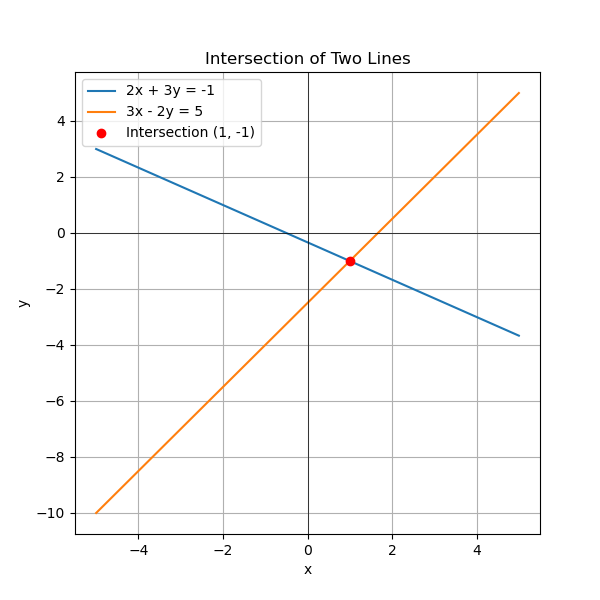
\includegraphics[width=0.7\columnwidth]{figs/fig1.png}
   \caption{}
   \label{Figure}
\end{figure}
    

\end{document}  